\documentclass{standalone}
\usepackage[dvipsnames]{xcolor}
\usepackage{tikz}
\usetikzlibrary{positioning, shapes, arrows,}

\begin{document}
\colorlet{DarkGreen}{Black!25!Green}
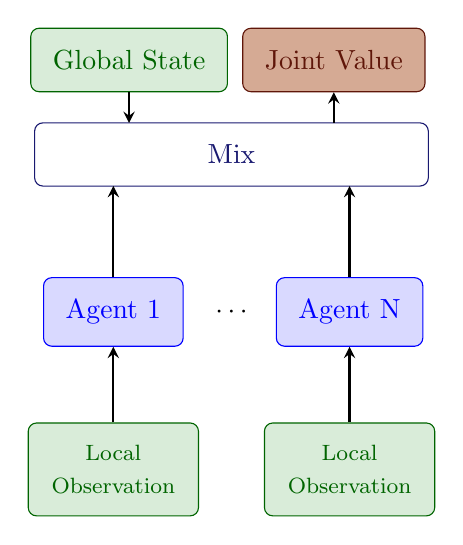
\begin{tikzpicture}[>=stealth, node distance=2cm, on grid, auto,
    entry/.style = {draw, rectangle, inner sep=8pt, rounded corners=3pt,
                    minimum width=1.5cm},
    greenEntry/.style = {draw, rectangle, inner sep=8pt, rounded corners=3pt,
                minimum width=1.5cm, align=center, DarkGreen, fill=Green!15},
    blueEntry/.style = {draw, rectangle, inner sep=8pt, rounded corners=3pt,
                    minimum width=1.5cm, Blue, fill=Blue!15},
    arrow/.style = {thick,-stealth}]

    % Entries
    \node [] (center) {\(\cdots\)};
    \node [blueEntry] (agent_1) [left =1.5cm of center] {Agent 1\ };
    \node [blueEntry] (agent_n) [right=1.5cm of center] {Agent N};
    \node [entry, MidnightBlue] (mix) [above=of center, minimum width=5cm] {Mix};
    \node [greenEntry] (state) [above left=1.2cm and 1.3cm of mix] 
        {Global State};
    \node [entry, Sepia, fill=Sepia!25] (value) [above right=1.2cm and 1.3cm of mix] {Joint Value};
    \node [greenEntry, text width=1.6cm] (obs_1) [below=of agent_1] 
        {\footnotesize Local Observation};
    \node [greenEntry, text width=1.6cm] (obs_n) [below=of agent_n] 
        {\footnotesize Local Observation};

    % Relations
    \draw [arrow] (obs_1) -- (agent_1);
    \draw [arrow] (obs_n) -- (agent_n);
    \draw [arrow] (agent_1) -- +(0,1.6);
    \draw [arrow] (agent_n) -- +(0,1.6);
    \draw [arrow] (state) -- +(0,-0.8);
    \draw [arrow] (value)+(0,-0.8) -- (value) ;
\end{tikzpicture}


\end{document}